\chapter{Fuerzas centrales} 
\refstepcounter{subsection}
Llamamos fuerza central a toda fuerza $\mathbf{F}(\mathbf{r})=F(\mathbf{r}) \hat{\mathbf{e}}_r \label{5.0.1} \inlineeqnum$, es decir, que ocurre en dirección radial a un punto determinado, si además esta fuerza central es conservativa, es equivalente a $\mathbf{F}(r)=F(r) \hat{\mathbf{e}}_r \label{5.0.2} \inlineeqnum$, es decir que es esférica simétricamente y solo depende de la distancia al origen, ya que
\[\mathbf{F}=F(r) \hat{\mathbf{e}}_r=-\nabla U(r,\theta,\varphi)=\frac{\partial U}{\partial r}\hat{\mathbf{e}}_r + \frac{1}{r}\frac{\partial U}{\partial \theta}\hat{\mathbf{e}}_\theta+\frac{1}{r\sin\theta}\frac{\partial U}{\partial \varphi}\hat{\mathbf{e}}_\varphi \implies \frac{\partial U}{\partial \theta}=\frac{\partial U}{\partial \varphi}=0\]
puesto que $1/r$ y $1/r\sin\theta$ no pueden ser 0, esto implica que $U=U(r)$ y $F=F(r)$, además llegamos a la siguiente expresión de $F$
\begin{equation} \label{5.0.3}
    F(r)=-\frac{\partial U}{\partial r}
\end{equation} \refstepcounter{subsection}
La recíproca, que $\mathbf{F}(r)=F(r) \hat{\mathbf{e}}_r$ es conservativa se puede obtener calculando su rotacional y verificando que es igual a 0.
\section{Problema de los dos cuerpos} \refstepcounter{subsection}
\begin{marginfigure}[-2cm]
    \def\svgwidth{125 pt}
    \tiny
	\input{images/centralf.pdf_tex}
	\labfig{margin2}
\end{marginfigure}
Si tenemos dos masas $m_1$ y $m_2$ con posiciones $\mathbf{r}_1$ y $\mathbf{r}_2$, de tal forma que sufren cada una una fuerza central conservativa creada por la otra masa, siguiendo la tercera ley de newton, entonces $U=U(r)$, donde $r=|\mathbf{r}_1-\mathbf{r}_2|=|\mathbf{r}| \label{5.1.1} \inlineeqnum$, tal que $\mathbf{r}=\mathbf{r}_1-\mathbf{r}_2 \label{5.1.2} \inlineeqnum$.

Podemos definir también el centro de masas del sistema de ambas masas, que se encuentra necesariamente en un punto intermedio entre ambas masas, y más cercano a la masa mayor
\begin{equation} \label{5.1.3}
    \mathbf{R} = \frac{1}{M}\sum^n{m_i \mathbf{r_i}} = \frac{m_1 \mathbf{r}_1 + m_2 \mathbf{r}_2}{m_1+m_2} \ \ \ \ \ M=\sum^n m_i
\end{equation} \refstepcounter{subsection}
De esta forma podemos hacer el cambio de las coordenadas $(\mathbf{r}_1,\mathbf{r}_2) \mapsto (\mathbf{r},\mathbf{R})$, que podemos invertir despejando $\mathbf{r}_1$ y de (5.1.2) y (5.1.3) e igualando para despejar $\mathbf{r}_2$, después sacamos $\mathbf{r}_1$ de una de las anteriores, tal que
\begin{equation} \label{5.1.4}
    \mathbf{r}_1 = \mathbf{R} + \frac{m_2}{M}\mathbf{r} \ \ \ \ \ \ \mathbf{r}_2 = \mathbf{R} - \frac{m_1}{M}\mathbf{r}
\end{equation} \refstepcounter{subsection}
Ahora podemos escribir $\pazocal{L}$ del sistema, para la energía cinética, veremos que los términos cruzados se cancelan
\begin{equation} \label{5.1.5}
    T=\frac{1}{2}m_1(\dot{\mathbf{r}}_1)^2+\frac{1}{2}m_2(\dot{\mathbf{r}}_2)^2=\frac{1}{2}M(\dot{\mathbf{R}})^2 + \frac{1}{2}\mu(\dot{\mathbf{r}})^2 \ \ \ \ \ 
    \boxed{\mu = \frac{m_1 m_2}{m_1+m_2}} \ \ \ \ \ \ \ U = U(r)
\end{equation} \refstepcounter{subsection}
\begin{equation} \label{5.1.6}
    \pazocal{L} = \pazocal{L}_{CM} + \pazocal{L}_{\mbox{\small rel}}= \left(\frac{1}{2}M(\dot{\mathbf{R}})^2\right) + \left(\frac{1}{2}\mu(\dot{\mathbf{r}})^2-U(r)\right)
\end{equation} \refstepcounter{subsection}
Es de notar que cuando la diferencia en las masas es muy grande, la masa reducida, $\mu$ tiende a la masa más pequeña.

De la ecuación (5.1.6) podemos concluir usando (E-L) que el momento asociado a $\mathbf{R}$ se conserva, puesto que que $\pazocal{L}$ no depende explícitamente de $\mathbf{R}$, entonces podemos llegar a tres ecuaciones resumidas en $M\ddot{\mathbf{R}}=0 \label{5.1.7} \inlineeqnum$, que indican que la velocidad del CM es constante.

Para el movimiento relativo en $\mathbf{r}$, aplicando (E-L), podemos llegar a tres ecuaciones que resuminos en $\mu\ddot{\mathbf{r}}=-\nabla U \label{5.1.8} \inlineeqnum$.

Entonces por (5.1.7), el sistema de referencia relativo al CM es un sistema inercial, de tal forma que estableciendo $\mathbf{R}=0$, podemos obtener las expresiones de $\mathbf{r}_1$ y $\mathbf{r}_2$ en el sistema del CM.
\begin{equation} \label{5.1.9}
    \mathbf{r}_1=\frac{m_2}{M}\mathbf{r} \ \ \ \ \ \mathbf{r}_2=-\frac{m_1}{M}\mathbf{r}
\end{equation} \refstepcounter{subsection}
Observando el dibujo de la página anterior, esta claro que en el sistema del CM, las posiciones de ambas masas deben estar en el mismo eje, es decir, sus vectores de posición son paralelos, puesto que $\mathbf{R}$ se encuentra siempre entre la recta que une a ambas masas.

Hay que tener cuidado por que $\mathbf{r}$ no es un vector posición, sino como definimos en (5.1.2), es la diferencia entre los dos vectores de posición.
\section{Conservación del momento angular}  \refstepcounter{subsection}
Definimos el momento angular total con respecto a O como $\mathbf{J} = \mathbf{J}_1 + \mathbf{J}_2 \label{5.1.10} \inlineeqnum$, donde $\mathbf{J}_i = \mathbf{r}_i \times \mathbf{p}_i = m_i \mathbf{r}_i \times \dot{\mathbf{r}}_i \label{5.1.11} \inlineeqnum$. La derivada del momento angular será entonces
\begin{equation} \label{5.1.12}
    \dot{\mathbf{J}_i}= m \left(\dot{\mathbf{r}}_i \times \dot{\mathbf{r}}_i + \mathbf{r}_i \times \ddot{\mathbf{r}}_i \right) = m \mathbf{r}_i \times \mathbf{r}_i = \mathbf{r}_i \times \mathbf{F}_i
\end{equation} \refstepcounter{subsection}
Entonces, usando la 3ª LN, (5.1.2) y (5.0.1), el momento angular total se conserva.
\begin{equation} \label{5.1.13}
    \dot{\mathbf{J}}=\mathbf{r}_1 \times \mathbf{F}_{12}+\mathbf{r}_2 \times \mathbf{F}_{21}=(\mathbf{r}_1-\mathbf{r}_2)\times \mathbf{F}=F \mathbf{r} \times \hat{\mathbf{u}}_r = 0
\end{equation} \refstepcounter{subsection}
El momento angular total en el sistema del CM es entonces, usando (5.1.9)
\begin{equation} \label{5.1.14}
    \mathbf{J} = \frac{m_1 m_2^2}{M^2} (\mathbf{r}\times \dot{\mathbf{r}})+ \frac{m_2 m_1^2}{M^2} (\mathbf{r}\times \dot{\mathbf{r}}) = \mu (\mathbf{r}\times \dot{\mathbf{r}})
\end{equation} \refstepcounter{subsection}
Como este se conserva puesto que sigue siendo inercial, esto implica que el movimiento de ambas masas debe ocurrir en un plano*, el perpendicular a $\mathbf{J}$.

Entonces podemos expresar la configuración del sistema con coordenadas polares, puesto que tenemos dos grados de libertad. Expresando el lagrangiano del sistema en coordenadas polares usando (5.1.6) y $\dot{\mathbf{r}}=d{(r \hat{\mathbf{u}}_r)}/dt=\dot{r}\hat{\mathbf{u}}_r + r \dot{\varphi}\hat{\mathbf{u}}_\varphi$ tenemos
\begin{equation} \label{5.1.15}
    \pazocal{L} = \frac{1}{2}\mu(\dot{\mathbf{r}})^2-U(r) = \frac{1}{2}\mu\left(\dot{r}^2+r^2\dot{\varphi}^2\right)-U(r)
\end{equation} \refstepcounter{subsection}
Vemos que entonces $\varphi$ es ignorable pues no aparece explícitamente y entonces su momento se conserva
\begin{equation} \label{5.1.16}
    p_\varphi = J = \frac{\partial \pazocal{L}}{\partial \dot{\varphi}} = \mu r^2 \dot{\varphi} \ \ \ \  \dot{p_\varphi} = 0
\end{equation} \refstepcounter{subsection}
Lo cual es exáctamente el módulo de $\mathbf{J}=\mu (r\hat{\mathbf{u}_r}\times (\dot{r}\hat{\mathbf{u}_r} + r \dot{\varphi} \hat{\mathbf{u}_\varphi}))= \mu r^2 \dot{\varphi}\hat{\mathbf{u}_z}$
\vspace{5pt}
\subsection{Esféricas *}
Podemos también demostrar que el movimiento ocurre en un plano escribiento el lagrangiano usando coordenadas esféricas, similar a (5.2.6), donde $\dot{\mathbf{r}}=d{(r \hat{\mathbf{u}}_r)}/dt=\dot{r}\hat{\mathbf{u}}_r + r \dot{\theta }\hat{\mathbf{u}}_\theta + r\sin \theta \dot{\varphi} \hat{\mathbf{u}}_\varphi$, tal que 
\begin{equation} \label{5.1.17}
    \pazocal{L} = \frac{1}{2}\mu(\dot{\mathbf{r}})^2-U(r) = \frac{1}{2}\mu\left(\dot{r}^2+r^2\dot{\theta}^2 + r^2 \sin^2 \theta \dot{\varphi}^2\right)-U(r)
\end{equation} \refstepcounter{subsection}
De esta forma vemos que $\varphi$ es la ignorable, de tal forma que su momento asociado se conservará
\begin{equation} \label{5.1.18}
    p_\varphi = \frac{\partial \pazocal{L}}{\partial \dot{\varphi}} = \mu r^2 \sin^2 \theta \dot{\varphi} \ \ \ \  \dot{p_\varphi} = 0
\end{equation} \refstepcounter{subsection}
Si ahora consideramos $\mathbf{J}$ en estas coordenadas usando (5.2.5)
\begin{equation} \label{5.1.19}
    \mathbf{J} = \mu (\mathbf{r} \times (\dot{r}\hat{\mathbf{u}}_r + r \dot{\theta}\hat{\mathbf{u}}_\theta + r\sin \theta \dot{\varphi} \hat{\mathbf{u}}_\varphi))=-\mu r^2 \sin \theta \dot{\varphi} \hat{\mathbf{u}}_\theta + \mu r^2 \dot{\theta}\hat{\mathbf{u}}_\varphi
\end{equation} \refstepcounter{subsection}
Como $\mathbf{J}$ se conserva, sus componentes se conservan, y entonces usando (5.2.10) en (5.2.9), verificamos que el movimiento ocurre en un plano, donde $\theta$ es constante.
\begin{equation} \label{5.1.20}
    p_\varphi = \mu r^2 \sin^2 \theta \dot{\varphi} = J_\theta \sin\theta \implies \frac{d}{dt} \sin\theta = \dot{\theta} \cos \theta = 0 \implies \dot{\theta} = 0
\end{equation} \refstepcounter{subsection}
\vspace{-30pt}
\subsubsection{Velocidad areolar}
Si consideramos el área que barre $\mathbf{r}$ en un pequeño incremento del tiempo como si fuera un triángulo, tenemos que, donde el primer término es la base del triángulo y el segundo la altura del triángulo, vemos que esta cantidad se conserva.
\begin{equation} \label{5.1.21}
    dA = \frac{1}{2} r\cdot r\dot{\varphi} dt \ \ \ \ \ \dot{A} = \frac{J}{2\mu} \ \ \ \ \ddot{A} = 0
\end{equation} \refstepcounter{subsection}
Esta ecuación se conoce como la segunda ley de \textit{Kepler}.
\section{Energía} \refstepcounter{subsection}
La energía (conservada e igual a $\pazocal{H}$), es, por (5.2.6) y (5.2.7)
\begin{equation} \label{5.1.22}
    E = T+U = \frac{1}{2}\mu\left(\dot{r}^2+r^2\dot{\varphi}^2\right)+U(r)=\frac{1}{2}\mu\dot{r}^2 + \frac{J^2}{2\mu r^2}+U(r)
\end{equation} \refstepcounter{subsection}
La ecuación (5.3.1) es una EDO de primer orden separable que nos permite hallar $r(t)$, invirtiendo la siguiente expresión
\begin{equation} \label{5.1.23}
    \int_{r_0}^r{\left[\frac{2}{\mu}\left(E-U(r)\right)-\frac{J^2}{\mu^2 r^2}\right]^{-\frac{1}{2}}dr}=t-t_0
\end{equation} \refstepcounter{subsection}

Usando (5.2.7) podemos encontrar $\varphi(t)$ una vez tenemos $r(t)$, de forma similar al formalismo Hamiltoniano.
\section{Ecuación del movimiento} \refstepcounter{subsection}
Haciendo (2.2.1)(E-L) con respecto a $r$ obtenemos la ecuación del movimiento del sistema
\begin{equation} \label{5.1.24}
    \mu \ddot{r} = \mu r \dot{\varphi}^2 - \frac{\partial U}{\partial r} = \frac{J^2}{\mu r^3}+ F(r)
\end{equation} \refstepcounter{subsection}

Nos va a interesar encontrar $r(\varphi)$ para no tener una expresión paramétrica de ambos sino la ecuación de una curva, para ello haremos el cambio de variable $u=1/r$.

Usando la regla de la cadena, el teorema de la función inversa y (5.1.16)
\begin{equation} \label{5.1.25}
    \frac{d u}{d\varphi}  = -\frac{1}{r^2} \frac{dr}{d\varphi} = -\frac{1}{r^2} \frac{dr}{dt} \frac{dt}{d\varphi}= -\frac{1}{r^2} \dot{r} \frac{1}{\frac{d\varphi}{dt}}=-\frac{1}{r^2} \dot{r} \frac{1}{\dot{\varphi}}= -\frac{1}{r^2} \dot{r} \frac{r^2 \mu}{J} = -\frac{\mu \dot{r}}{J}
\end{equation} \refstepcounter{subsection}
\begin{equation} \label{5.1.26}
    \frac{d^2 u}{d\varphi^2}  = \frac{d}{d\varphi}\left(-\frac{\mu \dot{r}}{J}\right)=-\frac{\mu}{J} \frac{d \dot{r}}{dt} \frac{dt}{d\varphi} = -\frac{\mu}{J} \frac{d \dot{r}}{dt} \frac{1}{\frac{d\varphi}{dt}} = -\frac{\mu}{J} \ddot{r} \frac{1}{\dot{\varphi}}= - \frac{\mu^2}{J^2} r^2 \ddot{r}
\end{equation} \refstepcounter{subsection}
Despejando $\ddot{r}$ de (5.4.3) y sustituyendo en (5.4.1) llegamos a la ecuación de la trayectoria, cuya solución es $r(\varphi)$
\begin{equation} \label{5.1.27}
    \frac{\partial^2 u}{\partial \varphi^2} + u = -\frac{\mu}{J^2 u^2}F(u) \iff \frac{\partial^2}{\partial \varphi^2}\left(\frac{1}{r}\right) + \frac{1}{r} = -\frac{\mu}{J^2}r^2F(r)
\end{equation} \refstepcounter{subsection}
\section{Potencial efectivo} \refstepcounter{subsection}
El primer término de la ecuación (5.4.1) se denomina fuerza centrífuga, a la que podemos asociar un potencial, tal que 
\begin{equation} \label{5.1.28}
    F_{\mbox{\small cf}} = \frac{J}{\mu r^3} = -\frac{\partial U_{\mbox{\small cf}}}{\partial r} \implies U_{\mbox{\small cf}} = \frac{J^2}{2\mu r^2}
\end{equation} \refstepcounter{subsection}
De esta forma las expresiónes (5.4.1) y (5.3.1) nos quedan
\begin{equation} \label{5.1.29}
    \mu \ddot{r} = -\frac{\partial}{\partial r} (U_{\mbox{\small cf}}+U) = -\frac{\partial U_{\mbox{\small ef}}}{\partial r} \ \ \ \ \ \  U_{\mbox{\small ef}} = U(r) + \frac{J^2}{2\mu r^2}
\end{equation} \refstepcounter{subsection}
\begin{equation} \label{5.1.29}
    E = \frac{1}{2}\mu \dot{r}^2 + \left(\frac{J^2}{2\mu r^2}+U(r)\right) = \frac{1}{2}\mu\dot{r}^2 + U_{\mbox{\small ef}}(r)
\end{equation} \refstepcounter{subsection}
El primer término de (5.5.3) lo llamamos el término cinético y siempre es positivo, esto implica necesariamente la siguiente relación que determinará que valores de $r$ podrá tomar el sistema.
\begin{equation} \label{5.1.30}
    E\geq U_{\mbox{\small uf}}(r) \ \ \forall t \ \ \ \ \ \ E = U_{\mbox{\small uf}}(r) \implies \dot{r}=0
\end{equation} \refstepcounter{subsection}


\clearpage
\section{Potenciales $-\gamma/r$}\refstepcounter{subsection}
Si tenemos un potencial de la forma siguiente, entonces el potencial efectivo asociado toma la siguiente expresión representada en la figura.
\begin{equation} \label{5.6.1}
    U(r) = -\frac{\gamma}{r} \ \ \ \ \gamma>0 \ \ \ \ \ \ U_{\mbox{\small ef}} =  \frac{J^2}{2\mu r^2} -\frac{\gamma}{r}
\end{equation} \refstepcounter{subsection}
\begin{figure}[h]
    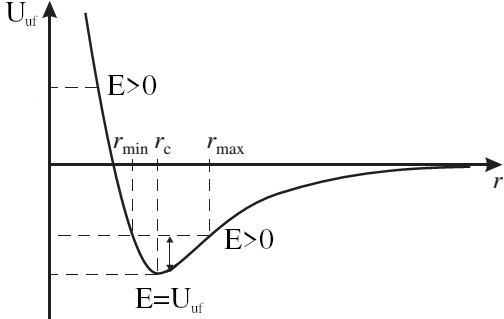
\includegraphics[width=12cm]{uf.png}
\end{figure}
Aplicando (5.5.4) podemos deducir ciertas propiedades del movimiento.

Si $E>0$, tenemos que la recta corta en un solo punto a $U_{\mbox{\small ef}}$, en ese punto serán iguales y la velocidad radial se anula. Esto nos indica que si r va disminuyendo, su velocidad radial es negativa pero su modulo va aumentando hasta que llega a $r_c$, donde la diferencia entre $E$ y $U_{\mbox{ \small ef}}$ es mayor y alcaza su pico, entonces el modulo de la velocidad radial disminuye hasta que se anula en el punto $r$ donde se cortan, entonces r volverá a aumentar, siendo su velocidad positiva y creciente, hasta alcanzar su pico en $r_c$, tras lo cual la velocidad decrece hasta un valor límite cuanto r tiende a infinito.

En cambio, si $E>0$, esta corta en dos puntos a $U_{ \mbox{\small ef}}$, donde la velocidad radial se anulará, lo que significa que $r$ esta acotado entre esos dos puntos $r_{\mbox{\small min}}$ y $r_{\mbox{\small max}}$, llamados \textit{periápside} y \textit{apoápside} respectivamente, entorno a los cuales oscilará, puesto que fuera de esa región no se cumple (5.5.4).

Estos valores pueden encontrarse igualando (5.6.1) a $E$ y resolviendo para $1/r$ como una ecuación cuadrática, obteniendo
\begin{equation} \label{5.6.2}
    \frac{1}{r}=\frac{\gamma \mu}{J^2}\left(1\pm\sqrt{1+\frac{2J^2 E}{\gamma^2 \mu}}\right)
\end{equation} \refstepcounter{subsection}

Diremos que una de trayectoria es cerrada cuando exista un periodo $\tau$ tal que $r(t+\tau)=r(t)$ y $\varphi(t+\tau)=\varphi(t) +2 \pi k$ para algún $k \in \mathbb{Z}$.

Si $E=U_{\mbox{\small ef}}$, la velocidad radial se anula y $r$ es constante, describiendo una órbita circular de radio $r_c$.

\section{Órbitas de Kepler} \refstepcounter{subsection}
Tenemos de nuevo $U(r)=-\gamma/r$ y $F(r)=-\gamma/r^2$ tal que $\gamma > 0$. Usando la ecuación de la trayectoria (5.4.4), tenemos que $F(u)=-\gamma u^2$, si $u=u(\varphi)$, entonces
\begin{equation} \label{5.7.1}
    u'' + \left(u -\frac{\mu \gamma}{J^2}\right) = 0 = u'' + \omega(\varphi) \rightarrow \omega'' = u'' \implies \omega'' + \omega = 0 
\end{equation} \refstepcounter{subsection}
Haciendo ese cambio de variable hemos encontrado una EDO facil de resolver, tal que , pudiendo escoger $\delta =0$ al escoger los ejes adecuados (el origen de $\varphi$)
\begin{equation} \label{5.7.2}
    \omega = A \cos{\varphi +\delta} \implies u(\varphi) = \omega + \frac{\mu \gamma}{J^2} = A \cos{\varphi} +\frac{\mu \gamma}{J^2} = \frac{\mu \gamma}{J^2}\left(1+ \frac{A J^2}{\mu \gamma} \cos(\varphi)\right)
\end{equation} \refstepcounter{subsection}
Renombrando ciertas constantes, usando que $A\geq0$ y sustituyendo $u$ llegamos a 
\begin{equation} \label{5.7.3}
    \frac{1}{c} = \frac{\mu \gamma}{J^2}>0 \ \ \ \ \epsilon=\frac{A J^2}{\mu \gamma}\geq 0 \ \ \ \ \ \ r(\varphi) = \frac{c}{1+\epsilon \cos\varphi}
\end{equation} \refstepcounter{subsection}
Veremos que (5.7.3) es la ecuación de las secciones cónicas en coordenadas polares.
\subsection{Caso $0 \leq \epsilon < 1 $}
Si $0 \leq \epsilon < 1 $, entonces el denominador de (5.7.3) nunca se anula, lo que significa que $r$ va a estar acotado con extremos $r_{\mbox{\small min}}$ y $r_{\mbox{\small max}}$ que ocurrirán en $\cos \varphi = \{1,-1\}$
\begin{equation} \label{5.7.4}
    r_{\mbox{\small min}}= \frac{c}{1+\epsilon} \ \ \ \ \ \ r_{\mbox{\small max}} = \frac{c}{1-\epsilon}
\end{equation} \refstepcounter{subsection}
Como el denominador no se anula, $r(\varphi+2\pi k)=r(\varphi)$ para cualquier $k\in \mathbb{Z}$, es decir es periódica en $\varphi$.

Si ahora expresamos (5.7.3) en cartesianas, primero definiendo las transformaciones
\begin{equation} \label{5.1.5}
    x = r\cos\theta \ \ \ \ y = r\sin \theta \ \ \ \ r^2=x^2+y^2
\end{equation} \refstepcounter{subsection}
\vspace{-15pt}
\begin{equation} \label{5.1.6}
    c = r +\epsilon r \cos\varphi = r+\epsilon x \rightarrow r = c-\epsilon x
\end{equation} \refstepcounter{subsection}
\vspace{-20pt}
\begin{equation} \label{5.1.7}
    (c-\epsilon x)^2 = c^2 + \epsilon^2 x^2 -2\epsilon c x = x^2 + y^2 \rightarrow x^2 +2 \frac{c\epsilon}{1-\epsilon^2}x +\frac{y^2}{1-\epsilon^2}=\frac{c^2}{1-\epsilon^2}
\end{equation} \refstepcounter{subsection}
Despejando c de (5.7.3) en (5.7.6), sustituyendo en (5.7.5) y operando llegamos a (5.7.7). Si ahora definimos las siguientes constantes
\begin{equation} \label{5.1.8}
    d = \frac{c\epsilon}{1-\epsilon^2} \ \ \ \ \ b^2 = \frac{c^2}{1-\epsilon^2} \ \ \ \ \ b^2 + d^2 = \frac{c^2}{(1-\epsilon^2)^2} = a^2
\end{equation} \refstepcounter{subsection}
\vspace{-15pt}
\begin{equation} \label{5.1.8}
    b^2 = a^2(1-\epsilon^2) \ \ (b<a) \ \ \ \ \ d=a\epsilon
\end{equation} \refstepcounter{subsection}
Podemos reescribir (5.7.7) y completar el cuadrado de $x$
\begin{equation} \label{5.1.7}
    x^2 +2dx +\frac{y^2}{1-\epsilon^2}=b^2 \rightarrow (x+d)^2 +\frac{y^2}{1-\epsilon^2}=b^2 + d^2 = a^2
\end{equation} \refstepcounter{subsection}
De esta forma pasando $a^2$ dividiendo y usando (5.7.9) obtenemos la ecuación de una elipse
\begin{equation} \label{5.1.7}
    \left(\frac{x+d}{a}\right)^2 +\left(\frac{y}{b}\right)^2=1
\end{equation} \refstepcounter{subsection}
\begin{figure}[H]
    \def\svgwidth{15 cm}
    \normalsize
	\input{images/orbit.pdf_tex}
	\labfig{margin2}
    \vspace{-75pt}
    \caption{Trayectoria $r(\varphi)$}
\end{figure}
\vspace{15pt}
Como se puede apreciar en (5.7.11), el centro de la elipse esta desplazado $d$ unidades hacía la derecha de $O$, la posición de $m_2$. Las constantes $a$ y $b$ son los semiejes mayor y menor respectivamente.

\subsubsection{Primera Ley de \texit{Kepler}}
Es importante notar que no estamos en el sistema del CM, sino en el sistema de $m_2$, aunque si la relación de masas es muy grade ambas posiciones son muy cercanas, de lo contrario siempre podemos usar (5.1.9) para obtener el moviemiento entorno al CM.

$m_2$ se encuentra en uno de los focos de la elipse por estar precisamente una distancia d del centro, esta es la primera ley de \texit{Kepler}.

\subsubsection{Excentricidad}
$\epsilon$ es la excentricidad de la elipse, podemos hallar una expresión de esta en función de $a$ y $b$ usando (5.7.9)
\begin{equation} \label{5.1.12}
    \epsilon = \sqrt{1-\frac{b^2}{a^2}}
\end{equation} \refstepcounter{subsection}
Cuando $a$ y $b$ son iguales tenemos un círculo y su excentricidad es 0, lo que implica que $r_{\mbox{\small min}} = r_{\mbox{\small max}}$.

Tenemos dos nuevas expresiones de los extremos $r_{\mbox{\small min}} = a (1-\epsilon) $ y  $r_{\mbox{\small max}} = a (1+\epsilon)$ usando (5.7.4) y (5.7.8).
\clearpage
\subsubsection{Periodo}
Como vimos en (5.2.12), la velocidad areolar es constante, lo que implica que el área total debe ser igual a la velocidad areolar por el periodo, tal que
\begin{equation} \label{5.1.13}
    a b \pi =A = \frac{J}{2 \mu} \tau
\end{equation} \refstepcounter{subsection}
Usando (5.7.3), (5.7.8) y (5.7.9) llegamos a 
\begin{equation} \label{5.1.14}
    \tau^2 = 4 \pi^2 \frac{\mu^2 a^2 b^2}{J^2} = 4 \pi^2 \frac{\mu^2 a^2 b^2}{c \gamma \mu} =  \frac{4 \pi^2  \mu}{\gamma} a^3
\end{equation} \refstepcounter{subsection}
Que dado $m_2 >> m_1$, entonces $\mu = m_1$ y si $\gamma = G m_1 m_2 $, (5.7.14) se transforma en la tercera ley de \texit{Kepler}.
\begin{equation} \label{5.1.14}
    \tau^2 =\frac{4 \pi^2}{G m_2} a^3
\end{equation} \refstepcounter{subsection}
\subsubsection{Energía}
Como la energía se conserva, podemos relacionar la energía con las constantes que hemos estado definiendo en un punto concreto de la trayectoria y se cumplirá para todos.
Para ello tomamos el caso del apoápside, donde la velocidad radial se anula.
\begin{equation} \label{5.1.14}
    E = \frac{J^2}{2\mu r_{\mbox{\small min}}^2}-\frac{\gamma }{r_{\mbox{\small min}}}
\end{equation} \refstepcounter{subsection}
Despejando $r_{\mbox{\small min}}$ de (5.7.4) y sustituyendo $c$ de (5.7.3) llegamos a 
\begin{equation} \label{5.1.14}
    r_{\mbox{\small min}} = \frac{J^2}{\gamma \mu (1+\epsilon)}
\end{equation} \refstepcounter{subsection}
Sustituyendo en (5.17.16) y operando llegamos a 
\begin{equation} \label{5.1.14}
    E = \frac{\gamma^2 \mu}{2 J^2} (\epsilon^2-1) \ \ \ \ \ \epsilon = \sqrt{1+\frac{2EJ^2}{\gamma^2 \mu}}
\end{equation} \refstepcounter{subsection}
Esta expresión se cumple para cualquier valor de $\epsilon$, lo que nos permite realcionar los valores de $\epsilon$ a las energías y relacionar con lo visto en (5.6), donde por ejemplo (5.6.2) es equivalente a las expresiones encontradas ahora.
\subsection{Caso $ç\epsilon = 1 $}
En este caso, el denominador se anula en $\cos \varphi = -1$, que ocurre cuando $\varphi$ tiende a $\pi$. Si de nuevo expresamos la ecuación (5.3.7) en cartesianas tenemos.
\begin{equation} \label{5.1.14}
    r = \frac{c}{1+\cos\varphi} \rightarrow r+x=c \rightarrow x^2+y^2 = (c-x)^2
\end{equation} \refstepcounter{subsection}
\vspace{-15pt}
\begin{equation} \label{5.1.14}
    y^2 = c^2 -2cx \rightarrow x = \frac{c^2 - y^2}{2c}
\end{equation} \refstepcounter{subsection}
Esta es la ecuación de una parábola en $y$ que se abre hacía la izquierda, cuando $\varphi$ tiende a $\pi$.
\subsection{Caso $ç\epsilon > 1 $}
En este caso, el denominador se anulará cuando $\cos \varphi = -1/\epsilon \label{5.1.7} \inlineeqnum$. Podemos aprovechar las mismas expresiones que en (5.7.11), pero teneiendo en cuenta que en (5.7.8) y (5.7.9), $1-\epsilon < 0$ y $1-\epsilon^2 < 0$, redefiniendo las constantes para que nos queden positivas tenemos
\begin{equation} \label{5.1.14}
    \delta = -d >0 \ \ \ \ \  \beta^2 = -b^2 >0 \ \ \ \ \alpha = -a>0
\end{equation} \refstepcounter{subsection}  
Tal que  (5.7.11) nos queda la ecuación de una hipérbola cuyas asíntotas verifican (5.7.21)
\begin{equation} \label{5.1.7}
    \left(\frac{x+d}{\alpha}\right)^2 -\left(\frac{y}{\beta}\right)^2=1
\end{equation} \refstepcounter{subsection}
\subsection{Cambio de Órbitas}
Vamos a suponer que partimos del periápside de una órbita, le damos un cierto impulso tangencial con $\mu$ y $\gamma$ constante, cambiando la órbita de $r_1(\varphi)$ a $r_2(\varphi)$, teniendo que
\begin{equation} \label{5.1.24}
    r_1(\varphi_0)=r_2(\varphi_0) \rightarrow \frac{c_1}{1+\epsilon_1 \cos(\varphi_0-\delta_1)} = \frac{c_2}{1+\epsilon_2 \cos(\varphi_0-\delta_2)}
\end{equation} \refstepcounter{subsection}
Como partimos del periápside, podemos escoger $\delta_1=0 \label{5.1.25} \inlineeqnum$ y entonces $\varphi_0=0 \label{5.1.25} \inlineeqnum$. Como el impulso es tangencial, es perpendicular a $\mathbf{r}_1$.

Esto solo ocurre para los extremos debido a la geometría de la elipse, esto implica entonces entonces que cuando cambiemos a la nueva órbita, también nos hallaremos en un extremo, pues la velocidad será perpendicular a $\mathbf{r}_2$, así $\delta_2=0 \label{5.1.25} \inlineeqnum$.

El impulso va a cambiar la velocidad de $v_1$ a $v_2$, y llamamos factor de impulso a $\lambda=v_2/v_1$, si $\lambda>1$, entonces la velocidad aumenta, si $\lambda < 1$, la velocidad disminuye.

Como la velocidad es perpendicular a $\mathbf{r}$, eso implica que $J_1=\mu r_1 v_1$ y $J_2=\mu r_2 v_2$, y haciendo despejando $\mu$ e igualando llegamos a $J_2 = \lambda J_1  \label{5.1.25} \inlineeqnum$.

Por otro lado, usando (5.7.3), la expresión de $c$, y (5.7.27), despejamos $\mu \gamma$ e igualamos y obtenemos $c_2= \lambda^2 c_1\label{5.1.25} \inlineeqnum$.

Ahora de (5.7.24) podemos despejar $\epsilon_2$ y susituimos (5.7.25-26-27) y (5.7.29)
\begin{equation} \label{5.1.24}
    \epsilon_2 = \lambda^2 \epsilon_1 + \lambda^2 -1
\end{equation} \refstepcounter{subsection}

Entonces si $\lambda >1$, tenemos que $\epsilon_2>\epsilon_1$, y entonces la órbita es mayor, si  $\lambda <1$, tenemos que $\epsilon_2<\epsilon_1$, y entonces la órbita es menor.